\documentclass[]{article}

\usepackage[nottoc,numbib]{tocbibind}

\usepackage{amssymb,amsmath}
\setcounter{tocdepth}{3}
\usepackage{graphicx}
\usepackage{algorithm, algorithmic}
\usepackage{caption}
\usepackage{complexity}
\usepackage{subcaption}
\usepackage{tabularx}
\usepackage{cite}
\usepackage{pgfgantt}
\usepackage{listings}
\usepackage{xcolor}
\definecolor{darkgreen}{rgb}{0.0, 0.5, 0.0}
\graphicspath{{images/}}
\captionsetup{compatibility=false}
\lstset{
    language=Python,
    basicstyle=\ttfamily\small,
    keywordstyle=\color{blue},
    stringstyle=\color{red},
    commentstyle=\color{darkgreen},
    showstringspaces=false,
    numbers=left,
    numberstyle=\tiny\color{gray},
    breaklines=true,
    frame=single,
    captionpos=b,
    emph={__init__}, % list function keywords or names here
    emphstyle=\color{purple} % set your preferred function name color here
}

%\usepackage{setspace}
%%\singlespacing
%%\onehalfspacing
%\doublespacing

\DeclareMathOperator*{\argmax}{argmax}

\DeclareMathOperator*{\optimise}{optimise}
\DeclareMathOperator*{\subjectto}{subject\hspace{0.1cm}to}
%opening
\title{\textbf{AI-Driven Generative Design: Evolutionary Optimization of Residential Floor Plans}}
\author{Zuxing Wu, a1816653\\ \\Supervisor: Adel Nikfarjam\\ \\Master of Computer Science}

\begin{document}

\maketitle\nonumber

\newpage\nonumber

\tableofcontents

\newpage

% \begin{abstract}
% Abstract
% \end{abstract}

\section{Introduction}
\subsection{Aim}
Residential floor plan design is a complex and challenging task that requires careful consideration of various factors, such as room sizes, adjacencies, privacy, convenience, and orientations. Traditional methods of floor plan design are often time-consuming and labor-intensive, leading to suboptimal solutions. Evolutionary algorithms have been proposed as a promising alternative for optimizing floor plans, as they can efficiently explore the design space and generate high-quality solutions. This project aims to develop a new method for optimizing residential floor plans using evolutionary algorithms and address some limitations of previous research. The proposed method will involve the application of evolutionary algorithms to generate and evolve floor plans based on a novel representation scheme. The fitness of each floor plan will be evaluated based on several criteria (e.g.\ privacy, comfort, practicality, convenience). The performance of the proposed method will be evaluated using a set of benchmark problems and compared with existing approaches. The results of this project will contribute to the field of residential floor plan design and provide valuable insights into the application of evolutionary algorithms to architectural design problems.

\subsection{Motivation}
Residential floor plan design is a critical aspect of architectural design that involves the layout of rooms, corridors, and other spaces within a building. The design of a floor plan can have a significant impact on the functionality, convenience, comfort, ventilation and energy efficiency of a building. Traditional methods of floor plan design are often based on manual sketches or computer-aided design (CAD) tools, which can be time-consuming and labor-intensive. Moreover, these methods may not always produce optimal solutions, as they rely on the intuition and experience of the designer.

Evolutionary algorithms have been proposed as a promising alternative for optimizing floor plans, as they can efficiently explore the design space and generate high-quality solutions. Evolutionary algorithms are a class of optimization algorithms inspired by the process of natural selection. They work by maintaining a population of candidate solutions (individuals) and iteratively applying genetic operators (e.g.,\ crossover, mutation) to generate new solutions. The fitness of each solution is evaluated based on predefined fitness functions, which measure how well the solution satisfies the objectives of the optimization problems.

\section{Literature Review}
Previous research has explored the application of evolutionary algorithms to optimize residential floor plans. Brintrup et al.~\cite{10.1007/11732242_56} compared three interactive genetic algorithms (i.e., sequential IGA, multi-objective IGA, parallel IGA) on a multi-objective floor planning task, and found that the multi-objective IGA provides more diverse results and faster convergence for optimizing floor plans. They developed interactive evolutionary algorithms that allow designers to incorporate their preferences and constraints into the optimization process. This method has shown promising results in generating floor plans that meet both functional and aesthetic requirements.

It was found that proportional roulette wheel selection is the best parent selection method for the mating pool, and k-point crossover is the most effective for fitness evolutionary improvement~\cite{7844659}.
Combining evolutionary algorithms with greedy-like algorithms can help find near-optimal solutions in Automated Floor Plan Generation (AFPG), though it is a simplified model of multi-objective optimization by linear composition of the partial evaluation functions~\cite{doi:10.1177/1478077119832982}. Subramanian et al.~\cite{9675541} used a genetic algorithm with KD tree models in a web application to generate floor plans for even non-expert users.

Wang and Duan~\cite{WANG2023100238} tried to optimize floor plan design by focusing on energy consumption and consumer satisfaction, proving that the preferences of different types of consumers differed significantly. Therefore, different evaluation criteria are needed for satisfying different family types~\cite{WANG2023100238}. The quality and efficiency of residential floor plan design can be improved by combining Monte Carlo tree search algorithm (MCTS) and particle swarm optimization (PSO)~\cite{YAN2024110546}. The MCTS algorithm takes human experience into consideration so that it can compress the search space and improve the efficiency of the search process~\cite{YAN2024110546}. The PSO algorithm can handle continuous variables and is suitable for optimizing the size of rooms due to parallel processing~\cite{YAN2024110546}.

Enengy consumption, probable uniformity (PU), and spatial useful daylight illuminance (sUDI) are three objectives that are considered in the optimization process using NSGA-II algorithm, and the results show that the NSGA-II algorithm can provide a set of more sustainable floor plans that requires less computational power and time~\cite{CHAICHI2024108842}. Reliable metrics for evaluating the amount of light and the uniformity of light are tested in the optimization process, and can avoid unwanted convergence because they restrict each other~\cite{CHAICHI2024108842}.

Furthermore, the integration of machine learning techniques with evolutionary algorithms has gained attention in recent decades. For example, Wang et al.~\cite{WANG20051329} proposed a hybrid approach that combines a genetic algorithm with a neural network to predict the fitness of candidate solutions. This method significantly reduces the computational cost of evaluating large populations and accelerates the optimization process.

Overall, the literature indicates that evolutionary algorithms, particularly when combined with other optimization techniques and machine learning methods, offer a powerful tool for optimizing residential floor plans. These approaches not only improve the efficiency and quality of the designs but also provide flexibility in accommodating various design preferences and constraints.

\section{Methodology}
The methodology of this project involves the application of evolutionary algorithms to optimize residential floor plans. The process will be divided into several key stages: initialization of the population, representation of the floor plan, design of the evolutionary optimization framework, and performance evaluation. These stages are outlined below.

\subsection{Population Initialization}
The first step in the evolutionary process is to generate an initial population of residential floor plans. An efficient initialization strategy will be employed to ensure diversity within the population while adhering to basic architectural constraints, such as room adjacency and size. Specifically, the initialization process will involve generating a set of random rooms and arranging them into a floor plan layout. The rooms will be assigned random sizes and positions within the layout, with constraints on room adjacencies and widths. The initialization strategy will be designed to produce a diverse set of floor plans that can serve as a starting point for the evolutionary optimization process.

\subsection{Representation of Floor Plans}
Residential floor plans will be represented using a Python class, that encodes the spatial information of rooms, such as adjacency and dimension. This representation will be designed to allow for easy manipulation by evolutionary operators (e.g.~crossover or mutation) while preserving architectural feasibility and obeying relevant constraints. Most importantly, the representation will be flexible enough to accommodate different types of rooms, such as bedrooms, living rooms, kitchens, and bathrooms. The representation will also include the presence of doors and windows, and other architectural features. This representation will be used throughout the optimization process to encode, decode, and evaluate floor plans.

\subsection{Evolutionary Optimization Framework}
The evolutionary optimization framework currently will be based on particle swarm optmization (PSO) algorithm, which is suitable for optimizing the size of rooms due to parallel processing~\cite{YAN2024110546}. The PSO algorithm will be used to evolve the population of floor plans over multiple generations. The framework will involve the application of genetic operators, such as crossover and mutation, to generate new floor plans from the existing population. The fitness of each floor plan will be evaluated based on 4 types of criteria (e.g.\ privacy, comfort, practicality, convenience). The optimization process will be repeated for a specified number of generations or until a termination criterion is met.

If possible, more than one evolutionary algorithms will be used in the process of optimizing the floor plan. For example, Monte Carlo tree search algorithm (MCTS) handles discrete variables (e.g.\ room position) and particle swarm optmization (PSO) deals with continuous variables~\cite{YAN2024110546}.

\subsection{Fitness Function Design}
The fitness function will evaluate each floor plan based on several criteria:
privacy, comfort, practicality, convenience.
These criteria can be evaluated by a group of human evaluators, shown as Table~\ref{table1}.
\begin{table}[h]
    \centering
    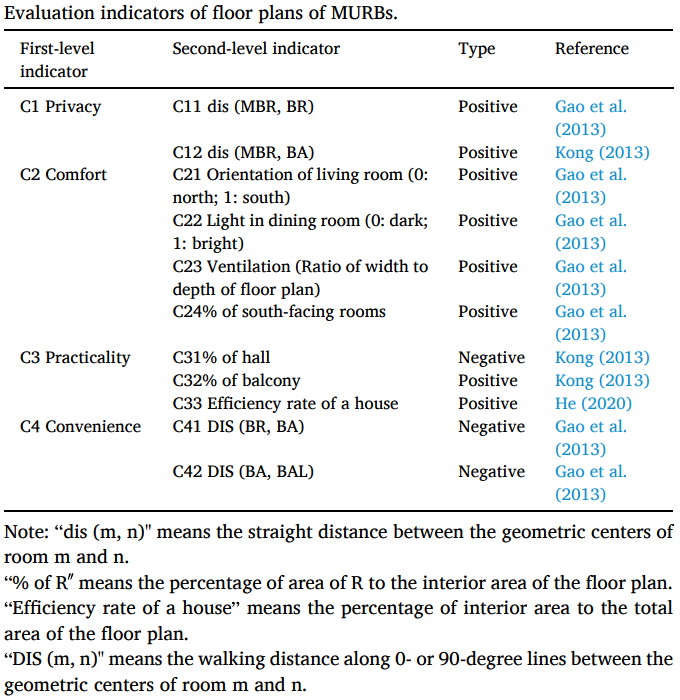
\includegraphics[width=0.8\textwidth]{image1.png}
    \caption{Evaluation indicators. Table 2 of Wang and Duan\cite{WANG2023100238}}\label{table1}
\end{table}

The straight distance between the geometric centers of room $m$ and $n$ is defined as:
\begin{equation*}
    \text{dis}(m, n) = \sqrt{(x_m - x_n)^2 + (y_m - y_n)^2}
\end{equation*}

The percentage of area of $R$ to the interior area of the floor plan is defined as:
\begin{equation*}
    \% \text{ of } R = \left( \frac{\text{Area of } R}{\text{Interior Area of Floor Plan}} \right) \times 100\%
\end{equation*}

The efficiency rate of a house is defined as the percentage of interior area to the total area of the floor plan:
\begin{equation*}
    \text{Efficiency Rate} = \left( \frac{\text{Interior Area}}{\text{Total Area}} \right) \times 100\%
\end{equation*}
The walking distance along 0- or 90-degree lines between the geometric centers of room $m$ and $n$ is defined as:
\begin{equation*}
    \text{DIS}_{\text{door}}(m, n) = \text{DIS}(m, \text{door}_m) + \text{DIS}(\text{door}_m, \text{door}_n) + \text{DIS}(\text{door}_n, n)
\end{equation*}


The proposed method will be implemented in Python. The optimization process will be carried out in two stages: initialization and mutation. The initialization stage will involve generating an initial population of floor plans using a novel strategy. The mutation stage will consist of iteratively applying genetic operators to the population to produce new generations. The fitness of each individual will be evaluated using multiple fitness functions that considers various factors such as the position of rooms, room sizes, and room adjacencies. The optimization process will be repeated for a specified number of generations or until a termination condition is met. The performance of the proposed method will be evaluated using a set of benchmark problems and compared with existing approaches.


\section{Plan vs Progress}
\subsection{Research Plan}
My research plan consists of four main phases at the end of the last semester:
\begin{itemize}
    \item Phase 1
          \begin{enumerate}
              \item Solution representation
              \item Solution evaluation
          \end{enumerate}
    \item Phase 2
          \begin{enumerate}
              \item Evolutionary optimization
              \item Population initialization
          \end{enumerate}
\end{itemize}
Each phase involves specific tasks and activities that will be carried out over a period of 6 months (since I did not make a plan for semester 1 of this year). The timeline for the research plan, at that time, is shown in the Gantt chart below. \\
\begin{ganttchart}[
        hgrid,
        vgrid,
        x unit = 1.4cm,
        y unit chart=0.7cm,
        title/.append style={fill=none},
        title label font=\bfseries\footnotesize,
        title label anchor/.append style={below=-1.6ex},
        include title in canvas=false,
        bar label font=\normalsize\scshape,
        bar label node/.append style={left=2ex},
        bar/.append style={fill=yellow!60},
        group/.append style={fill=cyan!80},
        bar incomplete/.append style={fill=red!30},
        progress label text={},
        group right shift=0,
        group top shift=0.7,
        group height=.3
    ]{1}{6}
    \gantttitle{2024.09--2025.02}{6} \\
    \gantttitlelist{9,10,11,12,1,2}{1} \\
    \ganttgroup{Phase 1}{1}{3} \\
    \ganttbar{Representation}{1}{2} \\
    \ganttbar{Evaluation}{2}{3} \\
    \ganttgroup{Phase 2}{4}{6} \\
    \ganttbar{Optimization}{4}{5} \\
    \ganttbar{Initialization}{5}{6}
    \gantttitle{Last Semester Research Plan Timeline}{6} \\
\end{ganttchart}

However, the real research progress did not go as planned. The research plan was adjusted to focus on the solution evaluation and evolutionary optimization. The solution evaluation is the key to the quality of generated floor plans, and the evolutionary optimization is the core of this research. The solution representation is the prerequisite of solution evaluation. The population initialization can be adjusted according to the progress of the research. The true timeline for the research progress is shown in the Gantt chart below. \\
\begin{ganttchart}[
        hgrid,
        vgrid,
        x unit = 1.0cm,
        y unit chart=0.7cm,
        title/.append style={fill=none},
        title label font=\bfseries\footnotesize,
        title label anchor/.append style={below=-1.6ex},
        include title in canvas=false,
        bar label font=\normalsize\scshape,
        bar label node/.append style={left=0.1ex},
        bar/.append style={fill=yellow!60},
        group/.append style={fill=cyan!80},
        bar incomplete/.append style={fill=red!30},
        progress label text={},
        group right shift=0,
        group top shift=0.7,
        group height=.3
    ]{1}{9}
    \gantttitle{2024.09--2025.05}{9} \\
    \gantttitlelist{9,10,11,12,1,2}{1}
    \gantttitlelist[title/.append style={fill=red!55}]{3,4,5}{1} \\
    \ganttgroup{Phase 1}{1}{3} \\
    \ganttbar{Representation}{1}{2} \\
    \ganttbar[bar/.append style={fill=brown!60}]{Evaluation}{2}{9} \\
    \ganttgroup{Phase 2}{4}{9} \\
    \ganttbar[bar/.append style={fill=brown!60}]{Optimization}{4}{9} \\
    \ganttbar{Initialization}{4}{7}
    \gantttitle{Real Research Progress}{9} \\
\end{ganttchart}


\subsection{Progress}
It can be seen from the Gantt chart above that the research process has been adjusted to mainly focus on the solution evaluation and evolutionary optimization.

Last summer holiday, I have completed the solution representation and solution evaluation, respectively using self-defined classes to represent the floor plan and using a set of fitness functions to evaluate each floor plan. All the fitness values are calculated and normalized to a range of 0 to 1.

Fitness functions are designed to evaluate the quality of the generated floor plans based on various criteria, such as privacy, comfort, practicality, and convenience. The evaluation process involves calculating the fitness values for each floor plan in the population and selecting the best individuals for particles updating their velocity and position in PSO.

\subsubsection{PSO algorithm + MCTS algorithm}
From the start of semester 1 of 2025, I have been working on the evolutionary optimization process. Initially, I focused on the PSO algorithm, which is suitable for optimizing the size of rooms due to parallel processing, and MCTS algorithm, which handles discrete variables (i.e., room position). I had implemented the PSO algorithm and MCTS algorithm in Python, and I tried integrating them into a single framework. The integration process involves combining the two algorithms to create a hybrid optimization approach that can effectively handle both continuous and discrete variables in the floor plan design process.

\subsubsection{MCTS algorithm replaced by (1+1) EA}
However, the integration process has proven to be more complex than anticipated, and the MCTS algorithm did not optimize the room position very well. Therefore, I changed it to a simple greedy algorithm called (1+1) Evolutionary Algorithm, which is a simple evolutionary algorithm that maintains a single individual and applies mutation to generate new individuals. The (1+1) EA algorithm is easier to implement and can be used to optimize the room position (i.e., the (x, y) coordinates) in the floor plan design process. If the new solution has a better fitness value, it replaces the current solution. This process continues until a termination criterion, such as a maximum number of iterations or a satisfactory fitness value, is met. It is a simple yet effective optimization algorithm that can be used to improve the quality of the generated floor plans, especially in terms of room position.

\subsubsection{Tune inertia weight}
In the PSO algorithm, the inertia weight plays a crucial role in balancing exploration and exploitation. Initially, I implemented a linearly decreasing inertia weight, which reduces the inertia weight from a maximum value to a minimum value over the course of iterations. However, after conducting experiments, I found that a non-linearly decreasing inertia weight performs better in terms of convergence speed and solution quality.

The non-linearly decreasing inertia weight is defined as:
\begin{equation*}
    w(t) = w_{\text{max}} + (w_{\text{min}} - w_{\text{max}}) \cdot \left(1 - \frac{t}{T}\right)^n
\end{equation*}
where $w(t)$ is the inertia weight at iteration $t$, $w_{\text{max}}$ and $w_{\text{min}}$ are the maximum and minimum inertia weights, $T$ is the total number of iterations, and $t$ is the current iteration. $t$ is the nonlinear modulation index in the range of [0.9, 1.3].

This non-linear decrease allows the algorithm to explore the search space more effectively in the early stages and focus on exploitation in the later stages. The quadratic term ensures a smoother transition, which helps in avoiding premature convergence and improves the overall performance of the optimization process.

\subsubsection{PSO algorithm replaced by (1+1) EA}
After that, we found that the PSO algorithm is not suitable for optimizing the size of rooms, because it always get trapped in a local optimum and can hardly break through it. Therefore, I changed it to (1+1) EA too, so that the room size (i.e., width and depth) can be optimized in a similar way to the room position mutation. The (1+1) EA algorithm will randomly select a room in the floor plan and generate a new room size by adding a small random perturbation to the current size. The new room size will be evaluated using the fitness functions, and if it results in a better fitness value, it will replace the current best room size. This process continues until all rooms have been assigned their optimal sizes.

\subsubsection{Swap two random rooms}
Through the above processes, swap mutation is used to optimize the room position. The swap mutation involves selecting two random rooms in the floor plan and swapping their positions. The swap mutation is a simple yet effective way to explore the design space and generate new floor plans. The new floor plans are evaluated using the fitness functions, and if they result in better fitness values, they will replace the current best floor plan.

\subsubsection{Prioritized fitness calculation}
To improve the performance of the optimization process, a prioritized fitness calculation strategy has been adopted. This strategy evaluates the fitness of floor plans based on the priority of the criteria, starting with the most important and moving to the less important ones. The prioritized fitness calculation process is outlined as follows:

\begin{enumerate}
    \item \textbf{Define Priorities:} Assign a priority level to each criterion (e.g., privacy, practicality, comfort, convenience). Higher priority criteria are evaluated first.
    \item \textbf{Sequential Evaluation:} Calculate the fitness values for each criterion in the order of their priority. For example, privacy is evaluated before practicality.
    \item \textbf{Weighted Aggregation:} Combine the fitness values using a weighted sum, where the weights correspond to the significance levels. The overall fitness value is given by:
          \begin{equation*}
              \text{Fitness}_{\text{total}} = \sum_{i=1}^{n} w_i \cdot \text{Fitness}_i
          \end{equation*}
          where $w_i$ is the weight for criterion $i$, and $\text{Fitness}_i$ is the fitness value for criterion $i$.
    \item \textbf{Early Termination:} If a floor plan fails to meet the minimum threshold for a high-priority criterion, it is discarded without evaluating the lower-priority criteria. This reduces unnecessary computations.
\end{enumerate}

This strategy ensures that the optimization process focuses on the most critical aspects of the floor plan design, improving both efficiency and the quality of the solution generation.
This approach allows for a more efficient evaluation process and helps to focus on the most critical aspects of the floor plan design, since it avoids unnecessary calculations in the early stages.

\subsubsection{Remove windows and doors}
In the previous version of the code, the windows and doors were added to each room immediately after the floor plan was generated. However, this approach led to a significant increase in the complexity of the optimization process, as the presence of windows and doors added additional constraints to the design. As a result, the optimization process became slower and less efficient, and the overall quality of the generated floor plans was not satisfactory even after multiple iterations.
To address this issue, I have removed the windows and doors from the early generation process. Instead, the optimization process will focus on generating the basic layout of the floor plan, including room sizes, positions, and an entry, without any additional features. Once the optimization process is completed and a satisfactory floor plan has been generated, windows and doors will be added to the final design. This approach simplifies the optimization process and allows for more efficient exploration of the design space.

\subsubsection{Change land size and orientation}
In the initial version of the code, the land size and orientation were fixed, which limited the flexibility of the design process. To enhance the adaptability of the floor plan generation, I have modified the code to allow for variable land sizes and orientations. This change enables the optimization process to spot potential problems and explore a wider range of design possibilities, accommodating different land configurations and orientations. The new approach allows for more diverse and flexible floor plan designs, making it easier to meet the needs and preferences of specific users.

\subsubsection{Dotted line for open space}
In the earlier design phase, the open space in the floor plan was represented by a solid line, which made it difficult to distinguish between open space and closed rooms. To improve the clarity of the design, I have changed the representation of open space to dotted lines. This change allows for a clearer visualization of the floor plan, making it easier to identify open spaces and their relationships with other rooms in the house.

\subsubsection{Tune weights}
To get satisfying floor plans, I keep tuning the weights of the fitness functions. The weights are used to balance the importance of different criteria in the evaluation process. By adjusting the weights, I can prioritize certain aspects of the design, such as low overlap or high utilization rate, to achieve better overall results. This tuning process is iterative and may require multiple rounds of testing and evaluation to find the optimal balance for the specific design goals.

\section{Experimental Results}


\section{Conclusion}


\section{Plagiarism Declaration}
I hereby declare that this submission is my own work and to the best of my knowledge, it contains no material previously published or written by another person, except where due to acknowledgment is made. Furthermore, I believe that it contains no material which has been accepted for the award of other degree or diploma in any university or other tertiary institutions.


\bibliographystyle{abbrv}
\bibliography{MyReferences}

\end{document}

